\documentclass[11pt,a4paper]{article}

\usepackage[margin=2.2cm]{geometry}
\usepackage[T1]{fontenc}
\usepackage[utf8]{inputenc}
\usepackage{lmodern}
\usepackage{microtype}
\usepackage{amsmath}
\usepackage{booktabs}
\usepackage{array}
\usepackage{longtable}
\usepackage{tabularx}
\usepackage{enumitem}
\usepackage{xcolor}
\usepackage{hyperref}
\usepackage{xurl}
\usepackage{tikz}
\usepackage{float}
\usepackage{listings}
\usetikzlibrary{arrows.meta,positioning,shapes.geometric,shapes.multipart,fit,calc}

\hypersetup{
  colorlinks=true,
  linkcolor=blue!50!black,
  urlcolor=blue!50!black
}

\newcommand{\placeholder}[1]{%
  \noindent\colorbox{yellow!20}{\parbox{\dimexpr\linewidth-2\fboxsep\relax}{\textbf{Placeholder to fill later:} #1}}%
}

\newcommand{\inlineplaceholder}[1]{\textcolor{orange!70!black}{[fill later: #1]}}
\newcommand{\codepath}[1]{\path{#1}}

\lstdefinestyle{codeblock}{
  basicstyle=\ttfamily\small,
  breaklines=true,
  breakatwhitespace=false,
  columns=fullflexible,
  keepspaces=true,
  showstringspaces=false
}

\title{\textbf{SLR Project P4 Report}\\Distributed MapReduce and Remote Experiment Infrastructure}
\author{Guilherme Caporali \and \inlineplaceholder{add teammate names if needed}}
\date{\today}

\begin{document}

\maketitle
\tableofcontents
\newpage

\section{Introduction}

This project comprises two distributed workflows executed over the Telecom
Paris laboratory machines: a custom MapReduce framework written in Go and a
deployment/collection pipeline used to launch programs remotely and gather
machine statistics. The principal engineering contribution is the MapReduce
system: the client builds a job-specific worker binary, deploys it to a pool
of remote hosts, distributes the input, drives map and reduce over HTTP, and
merges the final output locally.

The design objective was to remain compatible with the constraints of a
student laboratory environment: no root access, no Docker, shared machines,
SSH-based access only, and frequent host churn. The implementation therefore
relies on direct use of \texttt{/tmp}, SSH/SCP, HTTP, and bounded parallel
fan-out rather than on a more elaborate deployment stack.

\section{Overall architecture}

\subsection{System overview}

The repository contains two related but distinct distributed systems:

\begin{enumerate}[leftmargin=1.5em]
  \item \textbf{The MapReduce pipeline} exposed by \texttt{mapreduce.sh} and
  implemented mainly in \codepath{scripts/mapreduce}, \codepath{scripts/worker},
  and \codepath{scripts/jobs/*}.
  \item \textbf{The remote stats pipeline} exposed by \texttt{run.sh} and
  implemented in \codepath{scripts/make_hosts}, \codepath{scripts/deploy},
  \codepath{scripts/collect}, and \codepath{scripts/cleanup}.
\end{enumerate}

Both workflows share the same discovery model: the local machine first
queries \url{https://tp.telecom-paris.fr/ajax.php} to generate
\codepath{hosts.txt}, then fans out over SSH or HTTP to the selected nodes.

\begin{figure}[H]
\centering
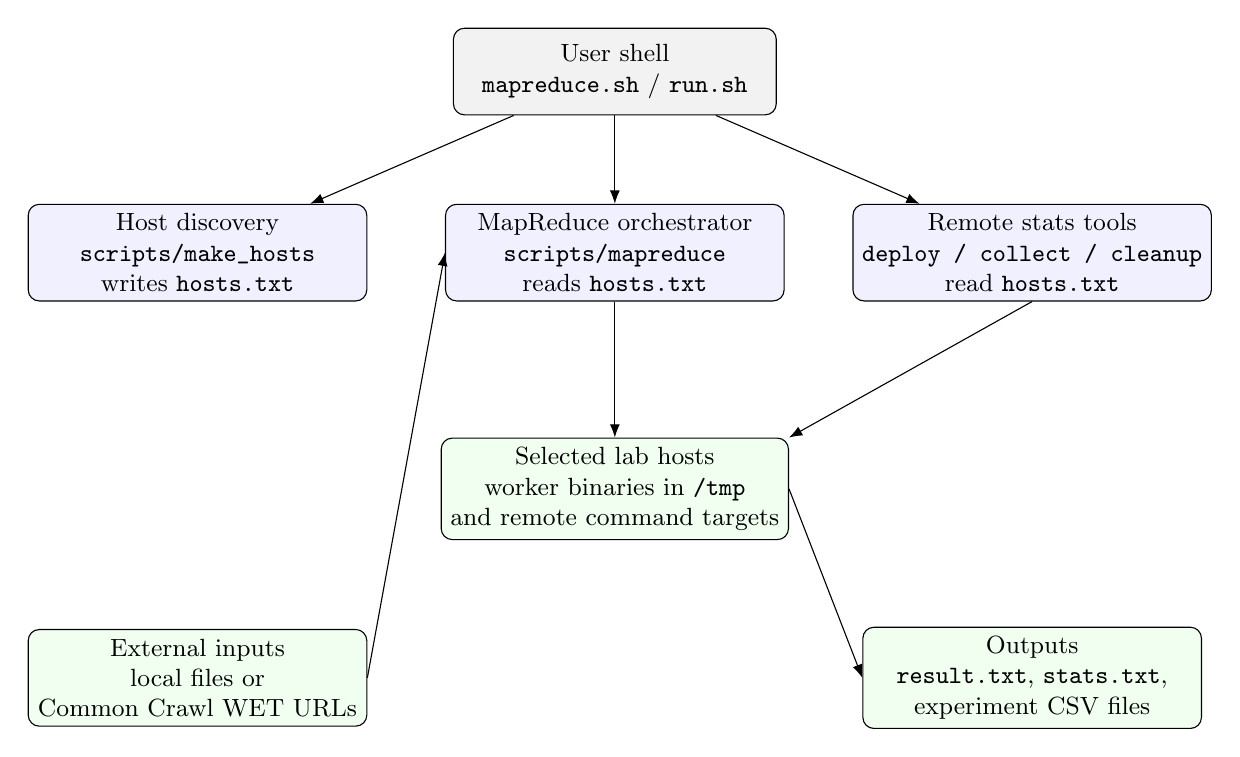
\begin{tikzpicture}[
  font=\small,
  box/.style={draw, rounded corners, align=center, minimum width=4.1cm, minimum height=1.1cm},
  service/.style={draw, rounded corners, fill=blue!6, align=center, minimum width=4.3cm, minimum height=1.1cm},
  data/.style={draw, rounded corners, fill=green!6, align=center, minimum width=4.3cm, minimum height=1.1cm},
  ->, >=Latex
]
  \node[box, fill=gray!10] (user) at (0,2.8) {User shell\\\texttt{mapreduce.sh} / \texttt{run.sh}};
  \node[service] (discover) at (-5.3,0.5) {Host discovery\\\codepath{scripts/make_hosts}\\writes \codepath{hosts.txt}};
  \node[service] (orchestrator) at (0,0.5) {MapReduce orchestrator\\\codepath{scripts/mapreduce}\\reads \codepath{hosts.txt}};
  \node[service] (stats) at (5.3,0.5) {Remote stats tools\\\texttt{deploy / collect / cleanup}\\read \codepath{hosts.txt}};
  \node[data] (machines) at (0,-2.5) {Selected lab hosts\\worker binaries in \texttt{/tmp}\\and remote command targets};
  \node[data] (inputs) at (-5.3,-4.9) {External inputs\\local files or\\Common Crawl WET URLs};
  \node[data] (outputs) at (5.3,-4.9) {Outputs\\\codepath{result.txt}, \codepath{stats.txt},\\experiment CSV files};

  \draw (user) -- (discover);
  \draw (user) -- (orchestrator);
  \draw (user) -- (stats);
  \draw (inputs.east) -- (orchestrator.west);
  \draw (orchestrator.south) -- (machines.north);
  \draw (stats.south) -- (machines.north east);
  \draw (machines.east) -- (outputs.west);
\end{tikzpicture}
\caption{Repository-level architecture. The MapReduce orchestrator and the
stats pipeline share the same host-discovery mechanism (\texttt{hosts.txt})
but execute different remote workflows on the lab machine pool.}
\end{figure}

\subsection{Main components}

\begin{longtable}{>{\raggedright\arraybackslash}p{2.6cm} >{\raggedright\arraybackslash}p{4.2cm} >{\raggedright\arraybackslash}p{7.8cm}}
\toprule
\textbf{Component} & \textbf{Location} & \textbf{Role} \\
\midrule
\endfirsthead
\toprule
\textbf{Component} & \textbf{Location} & \textbf{Role} \\
\midrule
\endhead
Wrapper scripts & \texttt{mapreduce.sh}, \texttt{run.sh} & User-facing entry points. They parse shell flags, fetch hosts, and launch the correct Go commands. \\
\addlinespace[0.35em]
Host discovery & \codepath{scripts/make_hosts} & Downloads the list of available lab machines and writes the first \(N\) hosts to \codepath{hosts.txt}. \\
\addlinespace[0.35em]
MapReduce orchestrator & \codepath{scripts/mapreduce} & Builds the worker binary for the selected job, deploys it, assigns input, coordinates phases, handles failures, and merges final results. \\
\addlinespace[0.35em]
Worker server & \codepath{scripts/worker} & Runs one HTTP server per host, stores local input and intermediate files, executes map and reduce, serves shuffle data, and exposes final results. \\
\addlinespace[0.35em]
Job API & \codepath{scripts/mrjob} & Defines the \texttt{Mapper} and \texttt{Reducer} interfaces used by all jobs. \\
\addlinespace[0.35em]
Jobs & \codepath{scripts/jobs/*} & Application logic. The repository already includes \texttt{wordcount}, \texttt{langdetect}, \texttt{domainpop}, and \texttt{docdensity}. \\
\addlinespace[0.35em]
Remote execution helpers & \codepath{scripts/internal/remote} & Provides bounded parallelism and shared SSH/SCP settings such as connection reuse and timeouts. \\
\addlinespace[0.35em]
Stats pipeline & \texttt{scripts/deploy}, \texttt{collect}, \texttt{cleanup} & Starts remote programs on many nodes, collects command outputs, and performs cleanup. \\
\addlinespace[0.35em]
Kafka comparison setup & \texttt{kafka/*} & Separate benchmark path used to compare the custom system with Kafka Streams on the same machine pool. \\
\bottomrule
\end{longtable}

\subsection{Detailed architecture of the MapReduce system}

The MapReduce architecture follows a client-orchestrated model rather than a
master that stays permanently deployed in the cluster.

\begin{enumerate}[leftmargin=1.5em]
  \item The local machine reads \texttt{hosts.txt} and decides how many hosts
  are active slots and how many are hot spares.
  \item The orchestrator cross-compiles a Linux worker binary that already
  contains the chosen job package. This is important: the remote worker does
  not dynamically load user code; the job is injected at build time.
  \item The binary is copied to every candidate node, then started with
  \texttt{nohup} as an HTTP server listening on the selected port.
  \item Input is assigned to slots. In local-file mode, the input is cut into
  chunks of at most 64 MB on newline boundaries. In Common Crawl mode, the
  orchestrator resolves WET URLs and distributes them round-robin.
  \item Each worker runs map locally and writes \(N\) intermediate bucket files
  to its node-local working directory in \texttt{/tmp}. The partition function
  is \(\mathrm{FNV32a}(key) \bmod N\).
  \item Each reducer then pulls exactly one bucket from each peer via HTTP,
  reconstructs the key groups in memory, applies the reducer, and exposes the
  final key/value lines at \texttt{/result}.
  \item The orchestrator collects every worker result, merges integer counts
  locally, sorts the final output, and writes the target file.
\end{enumerate}

Architecturally, the most important decision is that \textbf{\(N\) is fixed
for the whole job}. Since the partition function depends on \(N\), elasticity
is handled by replacing a failed \emph{host behind a logical slot} rather than
by changing the number of reducers in the middle of the run.

\section{Build, execution, and deployment}

\subsection{Prerequisites}

\begin{itemize}[leftmargin=1.5em]
  \item Go 1.25 or newer on the local machine.
  \item SSH key-based access to the Telecom Paris lab hosts.
  \item Network access to \texttt{tp.telecom-paris.fr}.
  \item For the Kafka comparison only: Java 17+ on the remote machines.
  \item On macOS, SSH multiplexing uses a control socket under \texttt{/tmp} to
  avoid Unix socket path-length limitations.
\end{itemize}

\subsection{How to run the project}

\subsubsection*{MapReduce pipeline}

\begin{lstlisting}[style=codeblock]
./mapreduce.sh -job scripts/jobs/wordcount -input data/simple.txt -output result.txt -n 10 -port 9090
\end{lstlisting}

or, with Common Crawl input:

\begin{lstlisting}[style=codeblock]
./mapreduce.sh -job scripts/jobs/wordcount -commoncrawl -crawl CC-MAIN-2026-21 \
  -files-limit 4 -output result.txt -n 10 -port 9090
\end{lstlisting}

\subsubsection*{Stats collection pipeline}

\begin{lstlisting}[style=codeblock]
./run.sh
\end{lstlisting}

This command fetches hosts, starts an HTTP server on each selected machine,
collects \texttt{hostname}, \texttt{uptime}, and memory data, and performs
cleanup on exit.

The current repository state also adds the following operational material:

\begin{itemize}[leftmargin=1.5em]
  \item built-in jobs under \codepath{scripts/jobs/}:
  \texttt{wordcount}, \texttt{langdetect}, \texttt{domainpop}, and
  \texttt{docdensity};
  \item a dedicated job-model document at \codepath{docs/JOBS.md};
  \item a batch runner, \codepath{run_all_commoncrawl_jobs.sh}, for executing
  all built-in jobs against Common Crawl while writing per-job outputs, logs,
  and timing summaries under \codepath{run/commoncrawl_jobs/}.
\end{itemize}

\subsection{Deploy workflow for the remote stats pipeline}

The repository contains a second distributed workflow, distinct from the
MapReduce runtime, whose purpose is to deploy a simple program to many lab
machines, collect command outputs, and clean up deterministically. This path is
exposed by \texttt{run.sh} and implemented by the four tools
\codepath{scripts/make_hosts}, \codepath{scripts/deploy},
\codepath{scripts/collect}, and \codepath{scripts/cleanup}.

\subsubsection*{Step-by-step execution}

\begin{enumerate}[leftmargin=1.5em]
  \item \textbf{Host discovery.} \texttt{run.sh} calls
  \codepath{scripts/make_hosts} with the configured value of \texttt{N}. The
  tool queries the Telecom Paris availability endpoint and writes the selected
  host list into \codepath{hosts.txt}.
  \item \textbf{Deployment.} \codepath{scripts/deploy} parses
  \codepath{manifest.json}, optionally copies listed files to the configured
  NFS location, then opens bounded-parallel SSH sessions to the selected hosts
  and executes every command listed in \texttt{commands}. In the current
  repository state, this phase starts a Python HTTP server on each host and
  writes its PID to \texttt{/tmp/httpserver.pid}.
  \item \textbf{Collection.} \codepath{scripts/collect} reuses the same host
  list and manifest, reads \texttt{collect\_commands}, runs those commands over
  SSH on every host, and writes a host-by-host report to \codepath{stats.txt}.
  In the present configuration, the collected values are \texttt{hostname},
  \texttt{uptime}, and the first two lines of \texttt{free -m}.
  \item \textbf{Cleanup.} \codepath{scripts/cleanup} runs the
  \texttt{cleanup\_commands} from the manifest on each host and, when relevant,
  removes deployed files from the configured NFS destination. The shell wrapper
  installs this cleanup phase in a trap so that teardown is attempted even when
  earlier phases fail.
\end{enumerate}

\subsubsection*{Configuration role of \texttt{manifest.json}}

The deploy workflow is parameterized by \codepath{manifest.json}:

\begin{itemize}[leftmargin=1.5em]
  \item \texttt{n} limits how many hosts are used by the deploy, collect, and
  cleanup tools;
  \item \texttt{files} and \texttt{nfs} describe optional files to copy to a
  shared NFS destination before remote execution;
  \item \texttt{commands} defines what the deploy phase starts remotely;
  \item \texttt{collect\_commands} defines what is sampled during collection;
  \item \texttt{cleanup\_commands} defines how remote state is removed.
\end{itemize}

\subsubsection*{Operational properties}

Three implementation details are particularly important for the report:

\begin{enumerate}[leftmargin=1.5em]
  \item SSH and SCP fan-out are bounded by the shared parallelism helpers in
  \codepath{scripts/internal/remote}, which prevents the client from opening an
  excessive number of concurrent connections.
  \item Remote command batches are executed in one SSH session per host, with
  command strings joined by \texttt{\&\&}, so a command failure stops the rest of
  that host's sequence.
  \item The deploy workflow is intentionally generic: the current repository
  starts a Python HTTP server, but the same mechanism can launch any other
  program that can be described through the manifest.
\end{enumerate}

\subsection{Exactly what must be changed for another student login}

The MapReduce path is largely login-agnostic because it deploys the worker to
\texttt{/tmp/mr-worker} on each host and does not embed a username in the
wrapper script. The portability-sensitive points are therefore limited and can
be stated precisely:

\begin{enumerate}[leftmargin=1.5em]
  \item \textbf{\texttt{manifest.json}, field \texttt{n}.} If the stats
  pipeline is used, the number of targeted hosts in \texttt{manifest.json}
  should stay consistent with the shell variable \texttt{N} in
  \texttt{run.sh}. In the repository snapshot, \texttt{run.sh} sets
  \texttt{N=100} and \texttt{manifest.json} also has \texttt{"n": 100}.
  \item \textbf{\texttt{manifest.json}, field \texttt{nfs}.} The generic
  \texttt{deploy}/\texttt{cleanup} tools support copying files to an NFS
  destination of the form \texttt{user@host:/shared/path/}. If a student uses
  that feature, this field must be changed to their own login and path.
  In the current repository state it is intentionally empty because the
  provided stats pipeline does not need NFS.
  \item \textbf{\texttt{manifest.json}, fields \texttt{commands},
  \texttt{collect\_commands}, and \texttt{cleanup\_commands}.} These commands
  must match the program the student wants to run remotely. The current values
  start a Python HTTP server and remove its PID file.
  \item \textbf{Input/output paths passed to \texttt{mapreduce.sh}.} These are
  not hardcoded, so another student only changes the command-line arguments:
  \texttt{-job}, \texttt{-input} or \texttt{-commoncrawl}, \texttt{-output},
  \texttt{-n}, and optionally \texttt{-port}.
  \item \textbf{SSH environment.} The project assumes the student already has
  passwordless SSH configured for the lab machines. That requirement lives
  outside the repository, but it is the only truly user-specific prerequisite
  for the MapReduce path.
\end{enumerate}

The recommended validation procedure with another student account is as
follows:

\begin{enumerate}[leftmargin=1.5em]
  \item clone the repository under the second login;
  \item verify SSH access to the lab hosts;
  \item run \texttt{./mapreduce.sh} on a small local input;
  \item run \texttt{./run.sh} after checking that \texttt{run.sh} and
  \texttt{manifest.json} agree on the host count.
\end{enumerate}

\placeholder{Insert the actual second-student validation result here: student
login used, commands run, whether any user-specific path needed adjustment,
and final outcome.}

\section{Protocol and phase execution}

\subsection{Worker HTTP API}

\begin{center}
\scriptsize
\begin{tabularx}{\linewidth}{>{\raggedright\arraybackslash}p{2.3cm} >{\raggedright\arraybackslash}p{1.3cm} X}
\toprule
\textbf{Endpoint} & \textbf{Method} & \textbf{Role} \\
\midrule
\texttt{/health} & GET & Readiness and liveness probe. \\
\addlinespace[0.35em]
\texttt{/data} & POST & Receives one raw input payload in local-file mode. \\
\addlinespace[0.35em]
\texttt{/load} & POST & Receives a JSON list of Common Crawl URLs and downloads them locally. \\
\addlinespace[0.35em]
\texttt{/map} & POST & Runs map on the locally stored input and creates pre-partitioned bucket files. \\
\addlinespace[0.35em]
\texttt{/intermediate} & GET & Serves one reducer bucket from the local disk. \\
\addlinespace[0.35em]
\texttt{/reduce} & POST & Pulls one bucket from each peer and runs reduce. \\
\addlinespace[0.35em]
\texttt{/result} & GET & Returns the final key/value lines. \\
\addlinespace[0.35em]
\texttt{/debug/pprof/*} & GET & Optional profiling endpoints when workers are started with \texttt{-pprof}. \\
\bottomrule
\end{tabularx}
\end{center}

\subsection{MapReduce phase sequence}

\begin{figure}[H]
\centering
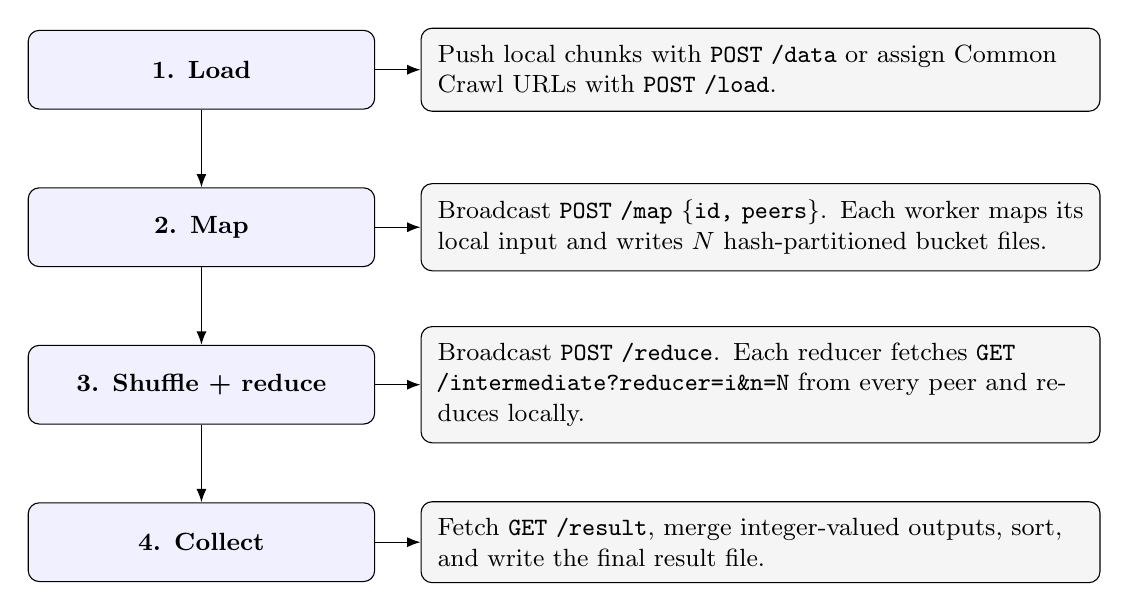
\begin{tikzpicture}[
  font=\small,
  stage/.style={draw, rounded corners, fill=blue!6, align=center, minimum width=4.4cm, minimum height=1.0cm},
  detail/.style={draw, rounded corners, fill=gray!8, align=left, text width=8.2cm, inner sep=6pt},
  ->, >=Latex
]
  \node[stage] (p1) at (0,0) {\textbf{1. Load}};
  \node[detail] (d1) at (7.1,0) {Push local chunks with \texttt{POST /data} or assign Common Crawl URLs with \texttt{POST /load}.};

  \node[stage] (p2) at (0,-2.0) {\textbf{2. Map}};
  \node[detail] (d2) at (7.1,-2.0) {Broadcast \texttt{POST /map \{id, peers\}}. Each worker maps its local input and writes \(N\) hash-partitioned bucket files.};

  \node[stage] (p3) at (0,-4.0) {\textbf{3. Shuffle + reduce}};
  \node[detail] (d3) at (7.1,-4.0) {Broadcast \texttt{POST /reduce}. Each reducer fetches \texttt{GET /intermediate?reducer=i\&n=N} from every peer and reduces locally.};

  \node[stage] (p4) at (0,-6.0) {\textbf{4. Collect}};
  \node[detail] (d4) at (7.1,-6.0) {Fetch \texttt{GET /result}, merge integer-valued outputs, sort, and write the final result file.};

  \draw[->] (p1) -- (p2);
  \draw[->] (p2) -- (p3);
  \draw[->] (p3) -- (p4);
  \draw[->] (p1.east) -- (d1.west);
  \draw[->] (p2.east) -- (d2.west);
  \draw[->] (p3.east) -- (d3.west);
  \draw[->] (p4.east) -- (d4.west);
\end{tikzpicture}
\caption{Single-job execution flow. The implementation has one MapReduce stage:
load, map, shuffle-by-pull, reduce, then result collection.}
\end{figure}

\noindent\textbf{Parallelism model:} All workers execute a given phase
concurrently. The orchestrator advances only after every active slot has
reached the required state for that phase.

\subsection{Input dispatch depending on dataset size and node count}

\subsubsection*{Local-file mode}

For a local input file, the orchestrator reads the whole file and splits it
into chunks of at most 64 MB, preferably on newline boundaries. This answers
the ``splitting'' part of the assignment: the split phase exists on the client
side before any remote computation starts.

In the current implementation, each slot receives at most one chunk through
\texttt{/data}. Concretely, slot \(i\) gets chunk \(i\), and if there are more
chunks than active slots, the extra chunks are not assigned in the current
\texttt{run()} path. Therefore:

\begin{itemize}[leftmargin=1.5em]
  \item if the file produces \(\leq N\) chunks, all data is dispatched;
  \item if the file produces \(> N\) chunks, the local-file path is at present
  incomplete and would need either round-robin multi-chunk assignment or a
  proper task scheduler.
\end{itemize}

This behavior is both a design characteristic and a significant remaining
limitation.

\subsubsection*{Common Crawl mode}

For Common Crawl, the orchestrator resolves a list of WET URLs and assigns them
round-robin across the \(N\) slots. Slot \(i\) receives URL indices
\(i, i+N, i+2N,\ldots\). Each worker then downloads its own files directly to
its local work directory. This mode does \emph{not} suffer from the one-chunk
per slot restriction because a worker may receive many URLs.

If \texttt{-files-limit} or \texttt{-chunks-limit} is lower than \(N\), some
workers may receive no URLs. The repository documentation now explicitly notes
this case and recommends increasing the Common Crawl limits or reducing
\(N\) when a more balanced assignment is required.

\subsubsection*{Dispatch rationale}

The dispatch strategy depends on the input type:

\begin{itemize}[leftmargin=1.5em]
  \item \textbf{Local file:} size-based chunking to keep request sizes bounded
  and preserve line boundaries.
  \item \textbf{Common Crawl:} URL-level round-robin distribution because the
  input is already segmented into remote WET files.
\end{itemize}

Round-robin distribution is straightforward and inexpensive to implement, but
it assumes that the remote files are broadly comparable in size. If some WET
files are substantially larger than others, the cluster remains susceptible to
input skew.

\subsection{Timing of each phase}

The implementation measures and logs the compute phases after the data has
already been loaded onto the workers:

\begin{itemize}[leftmargin=1.5em]
  \item load or upload is executed first and is excluded from the main
  \texttt{TIMING compute\_seconds=...} line;
  \item map, reduce, and result collection are timed explicitly;
  \item final local merge is part of result collection from the user point of
  view, but the code reports the \texttt{collect\_seconds} window separately
  from the total compute window.
\end{itemize}

There is \textbf{no second MapReduce stage} in the current implementation.
The workflow is a single-stage MapReduce job. If an application requires two
consecutive analytical passes, they must presently be executed as two separate
jobs.

\begin{table}[H]
\centering
\begin{tabular}{l c}
\toprule
\textbf{Phase} & \textbf{Status in current report} \\
\midrule
Client-side splitting & \inlineplaceholder{insert measured time} \\
\addlinespace[0.35em]
Input load / upload & \inlineplaceholder{insert measured time} \\
\addlinespace[0.35em]
Map & \inlineplaceholder{insert measured time} \\
\addlinespace[0.35em]
Shuffle & \inlineplaceholder{derive or estimate from logs / profiling} \\
\addlinespace[0.35em]
Reduce & \inlineplaceholder{insert measured time} \\
\addlinespace[0.35em]
Result collection and merge & \inlineplaceholder{insert measured time} \\
\addlinespace[0.35em]
Second MapReduce stage & Not applicable in the current design \\
\bottomrule
\end{tabular}
\caption{Required phase breakdown. The code already emits timings for map,
reduce, collect, and total compute; split and load can be measured around the
wrapper or orchestrator.}
\end{table}

\section{Project status: achieved functionality, unmet objectives, and remaining issues}

\subsection{Achieved}

\begin{itemize}[leftmargin=1.5em]
  \item A distributed MapReduce framework in Go, deployable on shared
  lab machines without root privileges.
  \item Pluggable job logic via a small \texttt{Mapper}/\texttt{Reducer} API.
  \item Support for both local files and Common Crawl WET inputs.
  \item A pull-based shuffle built on pre-partitioned bucket files.
  \item Bounded parallel SSH/SCP fan-out for deployment, collection, and
  cleanup.
  \item Fault handling through a slot-based coordinator with spare hosts,
  replacement, epoch tracking, and active health checks.
  \item Experiment scripts for Amdahl-law benchmarking and deployment-path
  benchmarking.
  \item A separate Kafka Streams benchmark path to support a system-level
  comparison.
\end{itemize}

\subsection{Outstanding items}

\begin{itemize}[leftmargin=1.5em]
  \item Fully general local-file scheduling for datasets larger than the number
  of available slots times one chunk. The code contains a round-robin
  multi-chunk helper, but the main execution path presently assigns only one chunk
  per slot.
  \item A fully populated empirical section in the report. The repository
  contains the scripts and plotting support, but the actual measurements remain
  to be produced and inserted.
  \item Durable storage or replicated intermediate data. The system is a batch
  engine, not a persistent data platform.
  \item Multi-stage job chaining inside one execution graph.
\end{itemize}

\subsection{Validated job executions recorded in the repository}

The current repository documentation now includes concrete single-worker
protocol validation results for the three analytical jobs added beyond word
count. These executions used the actual worker HTTP pipeline locally
(\texttt{/data} \(\rightarrow\) \texttt{/map} \(\rightarrow\)
\texttt{/reduce} \(\rightarrow\) \texttt{/result}), thereby exercising the real
map/reduce code paths while excluding only remote SSH/SCP deployment.

\begin{center}
\small
\begin{tabularx}{\linewidth}{>{\raggedright\arraybackslash}p{2.2cm} >{\raggedright\arraybackslash}p{4.0cm} X}
\toprule
\textbf{Job} & \textbf{Recorded output} & \textbf{Interpretation} \\
\midrule
\texttt{langdetect} & \texttt{lang:en 15} & All 15 input lines were classified as English, which matches the reference corpus used in the documented validation run. \\
\addlinespace[0.35em]
\texttt{domainpop} & \texttt{example.com 2}, \texttt{golang.org 1}, \texttt{news.ycombinator.com 2} & The reducer preserved the expected domain counts from the synthetic WARC-style input used for validation. \\
\addlinespace[0.35em]
\texttt{docdensity} & \texttt{hist:len.00000-00079 15}, \texttt{stat:chars.alnum 386}, \texttt{stat:chars.other 73}, \texttt{stat:chars.total 459}, \texttt{stat:lines 15} & The derived metrics reported in the repository documentation are \texttt{avg\_line\_length = 30.600} and \texttt{alnum\_density = 0.840959}, confirming that the counter-based output contract is sufficient for post-processing. \\
\bottomrule
\end{tabularx}
\end{center}

These documented validation results do not replace the distributed benchmark
section of this report, but they do confirm that the new job implementations
remain consistent with the worker protocol and integer-valued merge contract.

\subsection{Remaining problems}

\begin{enumerate}[leftmargin=1.5em]
  \item \textbf{Scalability bottleneck in local-file mode:} at present the
  largest correct local dataset is limited by the one-chunk-per-slot behavior.
  \item \textbf{Memory pressure in map and shuffle:} workers materialize large
  in-memory maps and arrays before writing or serving buckets.
  \item \textbf{Serial final merge:} the orchestrator continues to merge and sort
  results on one machine.
  \item \textbf{No data replication:} if a slot fails and no spare host is
  available, the whole job fails.
  \item \textbf{Skew sensitivity:} URL round-robin is straightforward but does not account for
  the true byte size or complexity of each WET file.
\end{enumerate}

\section{Maximum dataset size achieved}

The empirical maximum dataset size should be reported from real experiments, so
the exact number is left as a placeholder below. However, the implementation
already reveals two distinct limits:

\begin{itemize}[leftmargin=1.5em]
  \item \textbf{Local-file mode:} the current path is only correct while the
  number of generated chunks does not exceed the number of active slots.
  Since the chunk size is 64 MB, the practical bound is approximately
  \(64 \text{ MB} \times N\) before the current scheduler must be improved.
  \item \textbf{Common Crawl mode:} there is no such one-chunk structural
  limit because workers can receive many URLs. The effective maximum depends on
  available worker disk space under \texttt{/tmp}, network time, and job
  duration.
\end{itemize}

\placeholder{Insert the largest dataset actually processed successfully:
dataset identity, total bytes, node count, job used, and whether the run was
local-file or Common Crawl based.}

\section{Fault tolerance and crash behavior}

\subsection{Slot-based recovery model}

The coordinator tracks each logical worker slot through the states
\texttt{pending -> loaded -> mapped -> reduced -> done}. A slot is not bound
permanently to one physical machine. If a host fails, the coordinator can
rebind the same slot number to a spare host, replay prerequisite phases, and
preserve the same global reducer count \(N\).

\begin{figure}[H]
\centering
\resizebox{0.68\linewidth}{!}{%
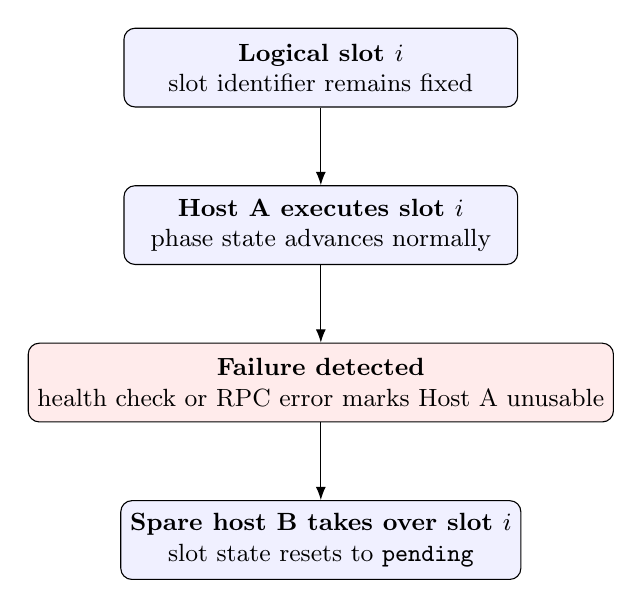
\begin{tikzpicture}[
  font=\small,
  phasebox/.style={draw, rounded corners, minimum width=5.0cm, minimum height=1.0cm, align=center, fill=blue!6},
  failurebox/.style={draw, rounded corners, minimum width=5.0cm, minimum height=1.0cm, align=center, fill=red!8},
  ->, >=Latex
]
  \node[phasebox] (s1) at (0,0) {\textbf{Logical slot \(i\)}\\slot identifier remains fixed};
  \node[phasebox] (s2) at (0,-2.0) {\textbf{Host A executes slot \(i\)}\\phase state advances normally};
  \node[failurebox] (s3) at (0,-4.0) {\textbf{Failure detected}\\health check or RPC error marks Host A unusable};
  \node[phasebox] (s4) at (0,-6.0) {\textbf{Spare host B takes over slot \(i\)}\\slot state resets to \texttt{pending}};

  \draw (s1) -- (s2);
  \draw (s2) -- (s3);
  \draw (s3) -- (s4);
\end{tikzpicture}
}
\caption{Alternative view of fault handling. The logical slot identifier is
preserved, while the physical host can be replaced and the necessary phases are
replayed before execution continues.}
\end{figure}

\noindent When a replacement occurs, the new host must replay the prerequisite
phases: it reloads the assigned input, reruns map, and only then rejoins the
current phase. If failure occurs after reduce has already run, the coordinator
bumps the epoch and invalidated reduces are recomputed against the updated peer
set.

\subsection{Failure scenario: node crash}

If a node crashes during the job:

\begin{enumerate}[leftmargin=1.5em]
  \item the health watcher polls \texttt{/health} periodically and marks a host
  as dead after consecutive failures;
  \item transport or HTTP errors during phase execution also identify a culprit
  slot or failing peer;
  \item the coordinator removes that host from future use and claims a spare;
  \item the replaced slot is reset to \texttt{pending}, so it reloads input and
  re-runs map before rejoining later phases;
  \item if the failure happened after reduce had already been completed by some
  workers, an epoch counter forces those reduce results to be recomputed because
  their previous peer set is now stale;
  \item if no spare host is available, the job stops with an explicit error.
\end{enumerate}

\subsection{Potential resilience improvements}

\begin{itemize}[leftmargin=1.5em]
  \item replicate intermediate buckets to another worker;
  \item checkpoint map completion and input assignment outside the process so
  recovery survives orchestrator crashes as well;
  \item replace in-memory state with a persistent metadata log;
  \item support multiple spare tiers or automatic host re-discovery;
  \item stream intermediate data so restart cost is lower for very large jobs.
\end{itemize}

\section{Threads, concurrency, and additional parallelization opportunities}

\subsection{Current use of threads}

In Go, the project uses goroutines rather than manual POSIX threads; however,
for the purposes of the assignment, these goroutines constitute the active
thread-level concurrency mechanism of the system.

\begin{center}
\begin{tabularx}{\linewidth}{>{\raggedright\arraybackslash}p{3.2cm} >{\raggedright\arraybackslash}p{4.0cm} X}
\toprule
\textbf{Location} & \textbf{Concurrent work} & \textbf{Reason} \\
\midrule
\codepath{scripts/internal/remote} & Bounded worker pools & Limit SSH/SCP fan-out while preserving parallel execution across many hosts. \\
\addlinespace[0.35em]
\codepath{scripts/deploy} & One goroutine per host copy/command batch & Reduce deployment latency across many machines. \\
\addlinespace[0.35em]
\codepath{scripts/collect} & Parallel SSH command execution & Reduce collection latency for remote statistics. \\
\addlinespace[0.35em]
\codepath{scripts/cleanup} & Parallel remote cleanup & Reduce shutdown time. \\
\addlinespace[0.35em]
\codepath{scripts/mapreduce} & Parallel deployment, health checks, phase broadcasts, result fetches & Drive all workers concurrently rather than serially. \\
\addlinespace[0.35em]
\codepath{scripts/mapreduce/coordinator.go} & One goroutine per slot in each pass; one health watcher thread & Advance slots independently and detect failures continuously. \\
\addlinespace[0.35em]
\codepath{scripts/worker} & One goroutine per peer during reduce fetch & Pull shuffle data from all peers concurrently. \\
\bottomrule
\end{tabularx}
\end{center}

\subsection{Areas where additional threads could be beneficial}

\begin{itemize}[leftmargin=1.5em]
  \item parallelizing map inside one worker across multiple local input files or
  independent line batches;
  \item parallelizing Common Crawl downloads per worker;
  \item streaming and decoding intermediate buckets concurrently instead of
  decoding each full JSON payload into memory first;
  \item parallelizing the final merge and sort on the orchestrator side.
\end{itemize}

\section{Storage, communication, and optimization opportunities}

\subsection{Memory or disk for intermediate results?}

The current design uses \textbf{both}, but for different stages:

\begin{itemize}[leftmargin=1.5em]
  \item during map, workers first build in-memory structures
  (\texttt{map[string][]string}) and only then partition them into bucket arrays;
  \item the partitioned intermediate output is then written to
  \textbf{node-local disk} under the worker's temporary directory;
  \item during reduce, the fetched intermediate buckets are read back into
  memory and regrouped by key before the reducer runs.
\end{itemize}

Accordingly, the authoritative copy of intermediate shuffle data resides on the
worker's local disk, not on NFS and not exclusively in RAM. This choice is
beneficial for avoiding NFS contention, although the current implementation
still uses more peak memory than necessary.

\subsection{FTP or sockets?}

The project does \textbf{not} use FTP.

\begin{itemize}[leftmargin=1.5em]
  \item host deployment and cleanup use SSH and SCP;
  \item MapReduce data exchange uses HTTP over TCP sockets;
  \item Common Crawl downloads also use HTTP;
  \item the stats pipeline collects command output over SSH.
\end{itemize}

\subsection{Optimization ideas}

\begin{enumerate}[leftmargin=1.5em]
  \item \textbf{Streaming map buckets:} write key/value lines directly to the
  target reducer files instead of materializing all reducer buckets in memory.
  \item \textbf{Streaming shuffle:} serve the \texttt{.jsonl} bucket files as a
  stream instead of decoding into an array and re-encoding them as JSON.
  \item \textbf{Combiner support:} for associative jobs such as word count, a
  local combiner would shrink the shuffle dramatically.
  \item \textbf{Better local-file scheduling:} use round-robin multi-chunk
  assignment or a true task queue so large inputs scale beyond \(N\) chunks.
  \item \textbf{Data-aware balancing:} weight Common Crawl files by size rather
  than by count only.
  \item \textbf{Parallel final merge:} the orchestrator can merge partial maps
  in parallel before sorting.
\end{enumerate}

\section{Experiments and results placeholders}

\subsection{Recommended experimental methodology}

The repository already contains the required experimental helpers:

\begin{itemize}[leftmargin=1.5em]
  \item \texttt{experiments/run\_benchmark.sh} for strong-scaling and
  Amdahl-law runs;
  \item \texttt{experiments/amdahl.gnuplot} to render the speedup plot;
  \item \texttt{experiments/run\_deploy\_benchmark.sh} to time
  deploy/collect/cleanup separately;
  \item the orchestrator log line
  \codepath{TIMING nodes=... map_seconds=... reduce_seconds=... collect_seconds=... compute_seconds=...}.
\end{itemize}

The report should use medians over multiple runs because the laboratory
machines are shared and therefore subject to performance variability.

\subsection{Results for different dataset sizes and node counts}

\begin{table}[H]
\centering
\resizebox{\linewidth}{!}{%
\begin{tabular}{l c c c c c}
\toprule
\textbf{Dataset} & \textbf{Bytes} & \textbf{Nodes} & \textbf{Median map (s)} & \textbf{Median reduce (s)} & \textbf{Median compute (s)} \\
\midrule
Small local test & \inlineplaceholder{fill} & 1 & \inlineplaceholder{fill} & \inlineplaceholder{fill} & \inlineplaceholder{fill} \\
\addlinespace[0.35em]
Small local test & \inlineplaceholder{fill} & 2 & \inlineplaceholder{fill} & \inlineplaceholder{fill} & \inlineplaceholder{fill} \\
\addlinespace[0.35em]
Common Crawl set A & \inlineplaceholder{fill} & 4 & \inlineplaceholder{fill} & \inlineplaceholder{fill} & \inlineplaceholder{fill} \\
\addlinespace[0.35em]
Common Crawl set B & \inlineplaceholder{fill} & 8 & \inlineplaceholder{fill} & \inlineplaceholder{fill} & \inlineplaceholder{fill} \\
\bottomrule
\end{tabular}
}
\caption{Placeholder table for the required experimental results over multiple
dataset sizes and machine counts.}
\end{table}

\placeholder{Replace the table above with the real median timings for all
dataset sizes and machine counts used in the final evaluation.}

\subsection{Amdahl's law: how to validate it empirically}

Yes, Amdahl's law can be validated empirically with this repository, provided
that the workload is kept fixed while the number of nodes changes. The supplied
\texttt{run\_benchmark.sh} script already implements the correct methodology:
it keeps one Common Crawl workload fixed and varies \(N\) over
\(\{1, 2, 4, 8, \ldots\}\).

\subsubsection*{What should be the speedup reference?}

The correct baseline is:

\[
S(N) = \frac{T(1)}{T(N)}
\]

where \(T(1)\) is the median runtime of the \textbf{same MapReduce algorithm}
on \textbf{the same dataset} with one active node. In other words:

\begin{itemize}[leftmargin=1.5em]
  \item the baseline should be the 1-node run, not the 2-node run;
  \item the algorithm should remain the custom MapReduce pipeline so that only
  cluster size changes;
  \item a comparison with a standard sequential algorithm remains useful, but
  it answers a different question than Amdahl scaling.
\end{itemize}

\subsubsection*{What graph shape should be expected?}

For a fixed dataset size, the speedup curve should generally:

\begin{enumerate}[leftmargin=1.5em]
  \item rise close to linearly for small \(N\);
  \item bend once communication, orchestration, and serial merge costs become
  significant;
  \item eventually flatten, because the serial fraction and shuffle overhead
  limit further gains.
\end{enumerate}

In this project, the main causes of deviation from ideal linear speedup are the
serial final merge, HTTP shuffle overhead, and skew across workers.

\subsubsection*{Should the graph be tried with multiple dataset sizes?}

Yes. Running the same node sweep for several dataset sizes is valuable because
the curve may change:

\begin{itemize}[leftmargin=1.5em]
  \item small datasets often saturate quickly because startup and communication
  dominate;
  \item larger datasets usually expose a higher effective parallel fraction
  because computation dominates fixed orchestration overheads longer.
\end{itemize}

\subsubsection*{Can the global parallel portion be deduced?}

Yes. Once the measured speedup curve is available, the global parallel portion
\(p\) can be estimated from Amdahl's law:

\[
S(N) = \frac{1}{(1-p) + \frac{p}{N}}
\]

By fitting the measured points, one can estimate \(p\) and therefore the
effective serial fraction \(1-p\).

\placeholder{Insert the measured speedup plot, fitted Amdahl curve, and the
estimated parallel portion \(p\). Also discuss whether the estimate changes
with dataset size.}

\subsection{Interpreting the phase breakdown}

The code naturally separates the following costs:

\begin{itemize}[leftmargin=1.5em]
  \item split and load cost before compute timing begins;
  \item map cost, which should scale best;
  \item shuffle cost, partly embedded in reduce because reducers pull from peers;
  \item reduce cost, which depends on key skew and network traffic;
  \item collection and final merge cost, which becomes increasingly serial.
\end{itemize}

The report should therefore comment not only on total runtime, but also on
which phase stops scaling first.

\section{Comparison with Kafka Streams}

\subsection{What is comparable}

The repository contains a Kafka benchmark path under \texttt{kafka/}:

\begin{itemize}[leftmargin=1.5em]
  \item \texttt{deploy\_kafka.sh} deploys Kafka brokers in KRaft mode;
  \item \texttt{WordCountJob.java} implements the word-count logic;
  \item \codepath{run_kafka_wordcount.sh} produces input, runs the job, and
  prints a \codepath{TIMING compute_seconds=...} line;
  \item \texttt{clean\_kafka.sh} removes the cluster state.
\end{itemize}

The appropriate comparison is to use the \textbf{same input file} and the
\textbf{same number of nodes} for both systems, then compare medians.

\subsection{Qualitative comparison}

\begin{center}
\begin{tabularx}{\linewidth}{>{\raggedright\arraybackslash}p{2.8cm} X X}
\toprule
\textbf{Aspect} & \textbf{Custom Go MapReduce} & \textbf{Kafka Streams} \\
\midrule
Execution model & Batch, phase-oriented job & Continuous stream processing on top of a persistent log \\
\addlinespace[0.35em]
Persistence & Intermediate data is local and temporary & Records are persisted in Kafka topics \\
\addlinespace[0.35em]
Fault tolerance & Spare-host replacement if available, but no durable replicated buckets & Built-in broker replication and consumer-group recovery \\
\addlinespace[0.35em]
Operational weight & Relatively light: Go binary + SSH + HTTP & More substantial: Java, Kafka brokers, topics, partitioning, cluster management \\
\addlinespace[0.35em]
Latency profile & Incurs per-phase orchestration and shuffle costs & Incurs per-record logging and streaming overhead \\
\addlinespace[0.35em]
Best fit & Batch analytics over temporary data & Durable, reusable, incrementally processed event streams \\
\bottomrule
\end{tabularx}
\end{center}

\subsection{Interpretation of the comparison}

Kafka is not simply ``superior'' or ``inferior.'' It addresses a broader
operational problem. It is expected to impose a larger operational footprint
because it offers persistent logs, partition management, and stronger recovery
semantics. The custom Go framework is lighter to understand and deploy for
batch experiments, but it relinquishes durability and a large portion of the
ecosystem support that Kafka provides.

Accordingly, the comparison may be summarized as follows:

\begin{itemize}[leftmargin=1.5em]
  \item the custom system is appropriate for experimentation and
  batch analytics under tight environment constraints;
  \item Kafka becomes preferable when the workload requires durable input
  retention, replay, incremental computation, or production-grade resilience.
\end{itemize}

\begin{table}[H]
\centering
\begin{tabular}{c c c c}
\toprule
\textbf{System} & \textbf{Nodes} & \textbf{Dataset} & \textbf{Median compute (s)} \\
\midrule
Go MapReduce & \inlineplaceholder{fill} & \inlineplaceholder{fill} & \inlineplaceholder{fill} \\
\addlinespace[0.35em]
Kafka Streams & \inlineplaceholder{fill} & \inlineplaceholder{fill} & \inlineplaceholder{fill} \\
\bottomrule
\end{tabular}
\caption{Placeholder for the required performance comparison with Kafka.}
\end{table}

\section{Conclusion}

The repository already contains a substantial distributed system: host
discovery, remote deployment, a pluggable MapReduce runtime, fault-aware slot
replacement, experiment scripts, and a Kafka comparison path. The architecture
is coherent for a lab setting because it deliberately avoids heavy external
dependencies and instead builds on SSH, HTTP, and node-local temporary storage.

The principal technical strengths are the simplicity of deployment, the clear
job API, and the slot-based recovery model. The principal weaknesses are the
one-chunk-per-slot limitation in local-file mode, memory-heavy map/shuffle
implementation, and the lack of durable replicated intermediate state.

\placeholder{Insert the final headline numbers here: maximum dataset size,
best speedup obtained, estimated parallel fraction, and the measured Kafka
comparison verdict.}

\appendix

\section{Reproducibility checklist}

\subsection{Core commands}

\begin{lstlisting}[style=codeblock]
# Run repository Go tests
cd scripts && go test ./...

# MapReduce on a local file
./mapreduce.sh -job scripts/jobs/wordcount -input data/simple.txt -output result.txt -n 10

# MapReduce on Common Crawl
./mapreduce.sh -job scripts/jobs/wordcount -commoncrawl -files-limit 10 -n 10 -output wc.txt

# Other provided jobs
./mapreduce.sh -job scripts/jobs/langdetect -commoncrawl -files-limit 10 -n 10 -output lang.txt
./mapreduce.sh -job scripts/jobs/domainpop  -commoncrawl -files-limit 10 -n 10 -output domains.txt
./mapreduce.sh -job scripts/jobs/docdensity -commoncrawl -files-limit 10 -n 10 -output density.txt

# Deployment/stats benchmark
experiments/run_deploy_benchmark.sh -n 100 -parallel-values "4 8 16 32" -reps 3

# Amdahl benchmark
experiments/run_benchmark.sh -job scripts/jobs/wordcount -chunks-limit 256 -reps 3

# Run all built-in jobs on Common Crawl
./run_all_commoncrawl_jobs.sh -crawl CC-MAIN-2026-21 -files-limit 1 -chunks-limit 1 -n 4

# Kafka comparison
(cd kafka && ./deploy_kafka.sh -n 10 && ./run_kafka_wordcount.sh -input /tmp/cc_split.txt && ./clean_kafka.sh)
\end{lstlisting}

\subsection{Docdensity post-processing}

\begin{lstlisting}[style=codeblock]
awk -F'\t' '$1=="stat:chars.total"{t=$2} $1=="stat:chars.alnum"{a=$2} $1=="stat:lines"{l=$2}
            END{printf "avg line len = %.1f chars\nalnum density = %.3f\n", t/l, a/t}' density.txt
\end{lstlisting}

\end{document}
